%!TEX TS-program = xelatex
\documentclass[10pt, compress]{beamer}

\usetheme[usetitleprogressbar]{m}

\usepackage{booktabs}
\usepackage{tikz}
\usepackage{dcolumn}
\usepackage[scale=2]{ccicons}
\usepackage{color}

\graphicspath{{Graphics/}}

\title[Tensors]{\textsc{Relax, Tensors Are Here...with Exogenous Covariates}}
\author[Hoff, Minhas, \& Ward]{Peter D. Hoff, Shahryar Minhas, \& Michael D. Ward} 
\date{\today}

\begin{document}
\frame{\titlepage}

%%%%%%%%%%%%%%%%%%%%%%%%%%%%%%%%%%%%%%%%%%%%%%%%%%%%%%%%%%%%
\frame
{
  \frametitle{Model Specification}
  \vspace{-5mm}
  \begin{itemize}
  \item Dependent variables: Log(Exports) and Stdzed(Material Conflict). 
  \item Direct ($i$), reciprocal ($ji$) and transitive ($ijk$) 1 month lags of these included as IVs.
  \item Exogenous Covariates:
    \begin{itemize}
    \item Number of Preferential Trade Agreements (PTA) between $i$ and $j$ (this is an undirected, yearly level variable). Direct and transitive version of this variable included as covariates.
    \item Presence of a defensive alliance relationship between $i$ and $j$ (undirected, yearly level). Direct and transitive versions.
    \item Centroid distance between $i$ and $j$ (directed). Direct version.
    \item Polity, monthly level variable. Polity of sender included.
    \item Log(GDP), yearly level variable but imputed at the monthly level. GDP of sender.
    \item Log(Population), yearly level variable but imputed at the monthly level. Population of sender.
    \item Log(Total Exports to any country), monthly level variable. Exports of sender.
    \end{itemize}
  \end{itemize}    
} 
%%%%%%%%%%%%%%%%%%%%%%%%%%%%%%%%%%%%%%%%%%%%%%%%%%%%%%%%%%%%

%%%%%%%%%%%%%%%%%%%%%%%%%%%%%%%%%%%%%%%%%%%%%%%%%%%%%%%%%%%%
\frame
{
  \frametitle{Sample \& Data}
  \begin{itemize}
  \item  Our sample is comprised of 161 countries over the period of March 2001 to December 2014
  \item Data sources:
  \begin{itemize}
    \item Exports: \href{http://data.imf.org/?sk=8aa6eb7c-598b-4d3b-82f4-adab95d23145&dsId=DS_1414779485682}{\textcolor{blue}{IMF Direction of Trade Statistics}}
    \item Material Conflict: ICEWS
    \item PTA: \href{http://www.designoftradeagreements.org/}{\textcolor{blue}{Design of Trade Agreements Database}}
    \item Alliance: \href{http://www.correlatesofwar.org/news/alliances-data-set-v4-1-available-1}{\textcolor{blue}{Correlates of War}}
    \item Distance: \href{http://nils.weidmann.ws/projects/cshapes}{\textcolor{blue}{cshapes}}
    \item Polity: \href{http://www.systemicpeace.org/polity/polity4.htm}{\textcolor{blue}{Polity IV Project}}
    \item GDP, Population: \href{https://www.imf.org/external/pubs/ft/weo/2014/02/weodata/index.aspx}{\textcolor{blue}{IMF World Economic Outlook Database}}
  \end{itemize}
  \end{itemize}    
} 
%%%%%%%%%%%%%%%%%%%%%%%%%%%%%%%%%%%%%%%%%%%%%%%%%%%%%%%%%%%%

%%%%%%%%%%%%%%%%%%%%%%%%%%%%%%%%%%%%%%%%%%%%%%%%%%%%%%%%%%%%
\frame
{
  \frametitle{Modeling Approach}
  \begin{itemize}
  \item Multilinear tensor regression framework
  \item MCMC run for 1300 iterations with first 600 used as burn-in\footnote{Using this many datapoints takes time the MCMC will keep running for another 3700 iterations so these results are preliminary, but trace plots at the end of this pdf look stable after 600 iterations}
  \item The model has the following form:
  \begin{align*}
  \textbf{Y} = \textbf{X} \times \{\boldsymbol{\beta_{1}}, \boldsymbol{\beta_{2}}, \boldsymbol{\beta_{3}} \} + \textbf{E}
  \end{align*}
  \item \textbf{Y} is a $161 \times 161 \times 2 \times 165$ array
  \item \textbf{X} is a $161 \times 161 \times 13 \times 165$ array, where each of the 13 variables is lagged by one month
  \end{itemize}    
} 
%%%%%%%%%%%%%%%%%%%%%%%%%%%%%%%%%%%%%%%%%%%%%%%%%%%%%%%%%%%%

%%%%%%%%%%%%%%%%%%%%%%%%%%%%%%%%%%%%%%%%%%%%%%%%%%%%%%%%%%%%
\frame
{
\frametitle{$\boldsymbol{\beta_{1}}$ \& $\boldsymbol{\beta_{2}}$, Sig. $+$ shown, $\alpha = 0.01$}
  \vspace{-15mm}
  \begin{figure}[ht]
  \centering
    \begin{tabular}{c}
      \includegraphics[width=1\textwidth]{net.pdf} \\
      \includegraphics[width=.9\textwidth]{map.pdf}
    \end{tabular}
  \end{figure}
}
%%%%%%%%%%%%%%%%%%%%%%%%%%%%%%%%%%%%%%%%%%%%%%%%%%%%%%%%%%%%

%%%%%%%%%%%%%%%%%%%%%%%%%%%%%%%%%%%%%%%%%%%%%%%%%%%%%%%%%%%%
\frame
{
\frametitle{$\boldsymbol{\beta_{3}}$}
  \centering
  \resizebox{1\textwidth}{!}{% Created by tikzDevice version 0.8.1 on 2015-06-28 20:26:01
% !TEX encoding = UTF-8 Unicode
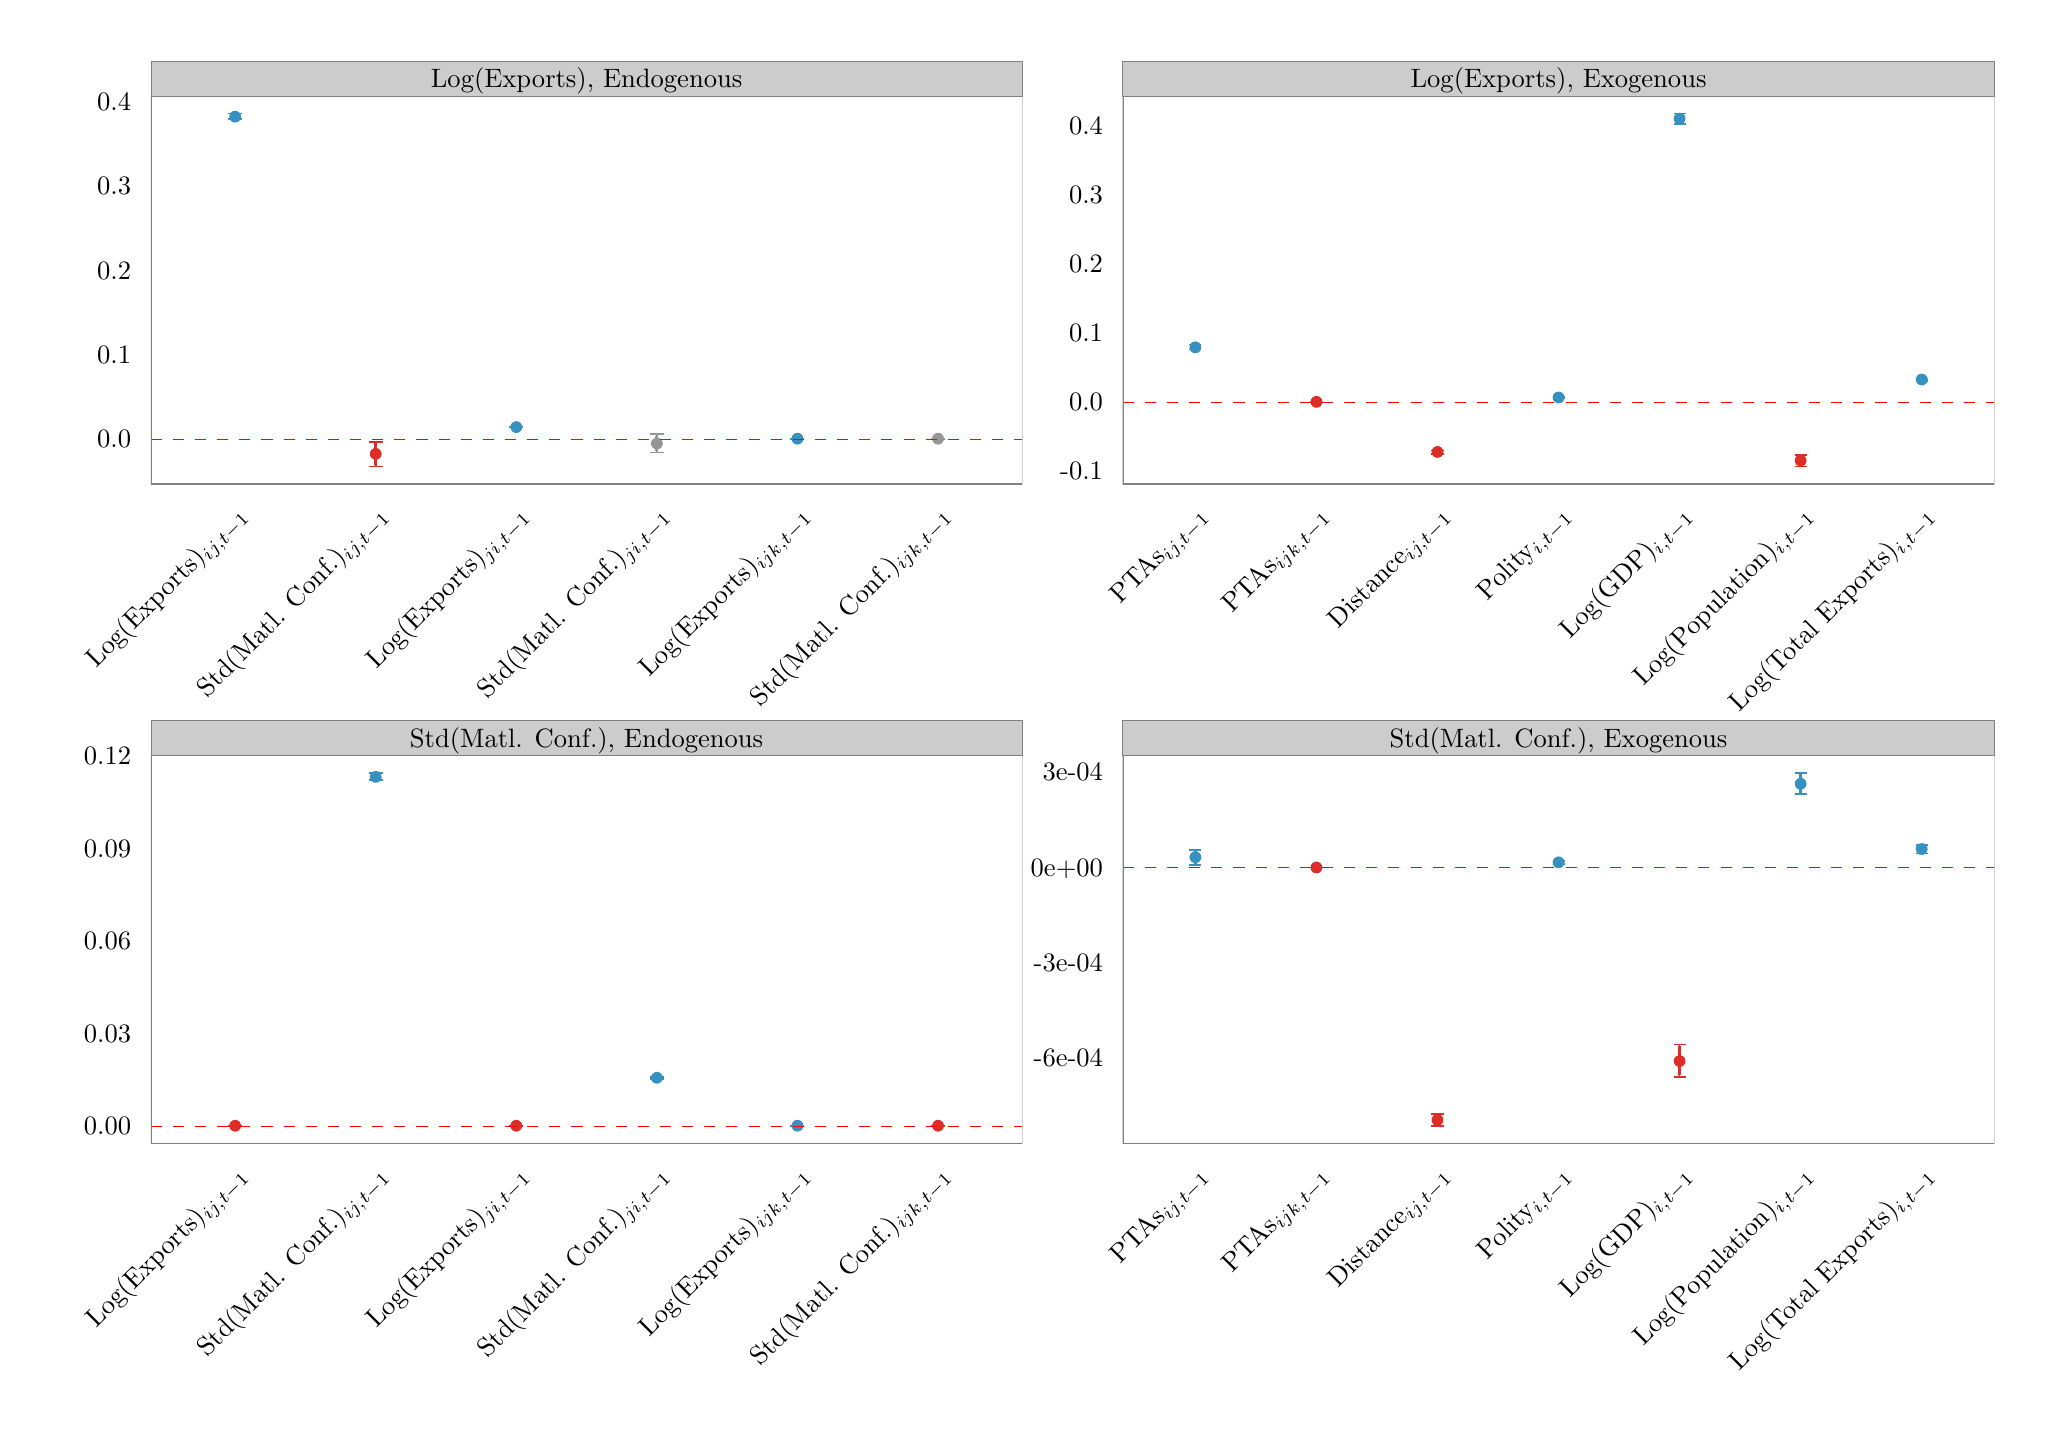
\begin{tikzpicture}[x=1pt,y=1pt]
\definecolor{fillColor}{RGB}{255,255,255}
\path[use as bounding box,fill=fillColor,fill opacity=0.00] (0,0) rectangle (722.70,505.89);
\begin{scope}
\path[clip] (  0.00,  0.00) rectangle (722.70,505.89);
\definecolor{drawColor}{RGB}{255,255,255}
\definecolor{fillColor}{RGB}{255,255,255}

\path[draw=drawColor,line width= 0.6pt,line join=round,line cap=round,fill=fillColor] (  0.00,  0.00) rectangle (722.70,505.89);
\end{scope}
\begin{scope}
\path[clip] ( 44.49,340.99) rectangle (359.44,481.21);
\definecolor{fillColor}{RGB}{54,144,192}

\path[fill=fillColor] ( 74.97,473.73) circle (  2.13);
\definecolor{fillColor}{RGB}{222,45,38}

\path[fill=fillColor] (125.77,351.89) circle (  2.13);
\definecolor{fillColor}{RGB}{54,144,192}

\path[fill=fillColor] (176.56,361.55) circle (  2.13);
\definecolor{fillColor}{gray}{0.59}

\path[fill=fillColor] (227.36,355.63) circle (  2.13);
\definecolor{fillColor}{RGB}{54,144,192}

\path[fill=fillColor] (278.16,357.36) circle (  2.13);
\definecolor{fillColor}{gray}{0.59}

\path[fill=fillColor] (328.96,357.36) circle (  2.13);
\definecolor{drawColor}{RGB}{54,144,192}

\path[draw=drawColor,draw opacity=0.30,line width= 0.3pt,line join=round] ( 74.97,472.79) -- ( 74.97,474.84);
\definecolor{drawColor}{RGB}{222,45,38}

\path[draw=drawColor,draw opacity=0.30,line width= 0.3pt,line join=round] (125.77,347.36) -- (125.77,356.18);
\definecolor{drawColor}{RGB}{54,144,192}

\path[draw=drawColor,draw opacity=0.30,line width= 0.3pt,line join=round] (176.56,361.43) -- (176.56,361.67);
\definecolor{drawColor}{RGB}{150,150,150}

\path[draw=drawColor,draw opacity=0.30,line width= 0.3pt,line join=round] (227.36,352.41) -- (227.36,359.04);
\definecolor{drawColor}{RGB}{54,144,192}

\path[draw=drawColor,draw opacity=0.30,line width= 0.3pt,line join=round] (278.16,357.36) -- (278.16,357.36);
\definecolor{drawColor}{RGB}{150,150,150}

\path[draw=drawColor,draw opacity=0.30,line width= 0.3pt,line join=round] (328.96,357.35) -- (328.96,357.37);
\definecolor{drawColor}{RGB}{54,144,192}

\path[draw=drawColor,line width= 1.1pt,line join=round] ( 74.97,472.86) -- ( 74.97,474.75);
\definecolor{drawColor}{RGB}{222,45,38}

\path[draw=drawColor,line width= 1.1pt,line join=round] (125.77,347.76) -- (125.77,355.64);
\definecolor{drawColor}{RGB}{54,144,192}

\path[draw=drawColor,line width= 1.1pt,line join=round] (176.56,361.45) -- (176.56,361.66);
\definecolor{drawColor}{gray}{0.59}

\path[draw=drawColor,line width= 1.1pt,line join=round] (227.36,352.95) -- (227.36,358.31);
\definecolor{drawColor}{RGB}{54,144,192}

\path[draw=drawColor,line width= 1.1pt,line join=round] (278.16,357.36) -- (278.16,357.36);
\definecolor{drawColor}{gray}{0.59}

\path[draw=drawColor,line width= 1.1pt,line join=round] (328.96,357.35) -- (328.96,357.37);
\definecolor{drawColor}{RGB}{54,144,192}

\path[draw=drawColor,line width= 0.6pt,line join=round] ( 72.43,474.84) --
	( 77.51,474.84);

\path[draw=drawColor,line width= 0.6pt,line join=round] ( 74.97,474.84) --
	( 74.97,472.79);

\path[draw=drawColor,line width= 0.6pt,line join=round] ( 72.43,472.79) --
	( 77.51,472.79);
\definecolor{drawColor}{RGB}{222,45,38}

\path[draw=drawColor,line width= 0.6pt,line join=round] (123.23,356.18) --
	(128.31,356.18);

\path[draw=drawColor,line width= 0.6pt,line join=round] (125.77,356.18) --
	(125.77,347.36);

\path[draw=drawColor,line width= 0.6pt,line join=round] (123.23,347.36) --
	(128.31,347.36);
\definecolor{drawColor}{RGB}{54,144,192}

\path[draw=drawColor,line width= 0.6pt,line join=round] (174.03,361.67) --
	(179.10,361.67);

\path[draw=drawColor,line width= 0.6pt,line join=round] (176.56,361.67) --
	(176.56,361.43);

\path[draw=drawColor,line width= 0.6pt,line join=round] (174.03,361.43) --
	(179.10,361.43);
\definecolor{drawColor}{gray}{0.59}

\path[draw=drawColor,line width= 0.6pt,line join=round] (224.82,359.04) --
	(229.90,359.04);

\path[draw=drawColor,line width= 0.6pt,line join=round] (227.36,359.04) --
	(227.36,352.41);

\path[draw=drawColor,line width= 0.6pt,line join=round] (224.82,352.41) --
	(229.90,352.41);
\definecolor{drawColor}{RGB}{54,144,192}

\path[draw=drawColor,line width= 0.6pt,line join=round] (275.62,357.36) --
	(280.70,357.36);

\path[draw=drawColor,line width= 0.6pt,line join=round] (278.16,357.36) --
	(278.16,357.36);

\path[draw=drawColor,line width= 0.6pt,line join=round] (275.62,357.36) --
	(280.70,357.36);
\definecolor{drawColor}{gray}{0.59}

\path[draw=drawColor,line width= 0.6pt,line join=round] (326.42,357.37) --
	(331.50,357.37);

\path[draw=drawColor,line width= 0.6pt,line join=round] (328.96,357.37) --
	(328.96,357.35);

\path[draw=drawColor,line width= 0.6pt,line join=round] (326.42,357.35) --
	(331.50,357.35);
\definecolor{drawColor}{RGB}{255,0,0}

\path[draw=drawColor,line width= 0.1pt,dash pattern=on 4pt off 4pt ,line join=round] ( 44.49,357.35) -- (359.44,357.35);
\definecolor{drawColor}{gray}{0.50}

\path[draw=drawColor,line width= 0.6pt,line join=round,line cap=round] ( 44.49,340.99) rectangle (359.44,481.21);
\end{scope}
\begin{scope}
\path[clip] (395.70,340.99) rectangle (710.66,481.21);
\definecolor{fillColor}{RGB}{54,144,192}

\path[fill=fillColor] (421.94,390.38) circle (  2.13);
\definecolor{fillColor}{RGB}{222,45,38}

\path[fill=fillColor] (465.69,370.67) circle (  2.13);

\path[fill=fillColor] (509.43,352.56) circle (  2.13);
\definecolor{fillColor}{RGB}{54,144,192}

\path[fill=fillColor] (553.18,372.27) circle (  2.13);

\path[fill=fillColor] (596.92,473.02) circle (  2.13);
\definecolor{fillColor}{RGB}{222,45,38}

\path[fill=fillColor] (640.66,349.47) circle (  2.13);
\definecolor{fillColor}{RGB}{54,144,192}

\path[fill=fillColor] (684.41,378.74) circle (  2.13);
\definecolor{drawColor}{RGB}{54,144,192}

\path[draw=drawColor,draw opacity=0.30,line width= 0.3pt,line join=round] (421.94,389.61) -- (421.94,391.34);
\definecolor{drawColor}{RGB}{222,45,38}

\path[draw=drawColor,draw opacity=0.30,line width= 0.3pt,line join=round] (465.69,370.66) -- (465.69,370.68);

\path[draw=drawColor,draw opacity=0.30,line width= 0.3pt,line join=round] (509.43,351.89) -- (509.43,353.15);
\definecolor{drawColor}{RGB}{54,144,192}

\path[draw=drawColor,draw opacity=0.30,line width= 0.3pt,line join=round] (553.18,372.13) -- (553.18,372.46);

\path[draw=drawColor,draw opacity=0.30,line width= 0.3pt,line join=round] (596.92,471.02) -- (596.92,474.84);
\definecolor{drawColor}{RGB}{222,45,38}

\path[draw=drawColor,draw opacity=0.30,line width= 0.3pt,line join=round] (640.66,347.36) -- (640.66,351.51);
\definecolor{drawColor}{RGB}{54,144,192}

\path[draw=drawColor,draw opacity=0.30,line width= 0.3pt,line join=round] (684.41,378.24) -- (684.41,379.14);
\definecolor{drawColor}{RGB}{54,144,192}

\path[draw=drawColor,line width= 1.1pt,line join=round] (421.94,389.74) -- (421.94,391.19);
\definecolor{drawColor}{RGB}{222,45,38}

\path[draw=drawColor,line width= 1.1pt,line join=round] (465.69,370.66) -- (465.69,370.68);

\path[draw=drawColor,line width= 1.1pt,line join=round] (509.43,352.02) -- (509.43,353.10);
\definecolor{drawColor}{RGB}{54,144,192}

\path[draw=drawColor,line width= 1.1pt,line join=round] (553.18,372.15) -- (553.18,372.40);

\path[draw=drawColor,line width= 1.1pt,line join=round] (596.92,471.12) -- (596.92,474.72);
\definecolor{drawColor}{RGB}{222,45,38}

\path[draw=drawColor,line width= 1.1pt,line join=round] (640.66,347.78) -- (640.66,351.37);
\definecolor{drawColor}{RGB}{54,144,192}

\path[draw=drawColor,line width= 1.1pt,line join=round] (684.41,378.33) -- (684.41,379.08);

\path[draw=drawColor,line width= 0.6pt,line join=round] (419.76,391.34) --
	(424.13,391.34);

\path[draw=drawColor,line width= 0.6pt,line join=round] (421.94,391.34) --
	(421.94,389.61);

\path[draw=drawColor,line width= 0.6pt,line join=round] (419.76,389.61) --
	(424.13,389.61);
\definecolor{drawColor}{RGB}{222,45,38}

\path[draw=drawColor,line width= 0.6pt,line join=round] (463.50,370.68) --
	(467.87,370.68);

\path[draw=drawColor,line width= 0.6pt,line join=round] (465.69,370.68) --
	(465.69,370.66);

\path[draw=drawColor,line width= 0.6pt,line join=round] (463.50,370.66) --
	(467.87,370.66);

\path[draw=drawColor,line width= 0.6pt,line join=round] (507.24,353.15) --
	(511.62,353.15);

\path[draw=drawColor,line width= 0.6pt,line join=round] (509.43,353.15) --
	(509.43,351.89);

\path[draw=drawColor,line width= 0.6pt,line join=round] (507.24,351.89) --
	(511.62,351.89);
\definecolor{drawColor}{RGB}{54,144,192}

\path[draw=drawColor,line width= 0.6pt,line join=round] (550.99,372.46) --
	(555.36,372.46);

\path[draw=drawColor,line width= 0.6pt,line join=round] (553.18,372.46) --
	(553.18,372.13);

\path[draw=drawColor,line width= 0.6pt,line join=round] (550.99,372.13) --
	(555.36,372.13);

\path[draw=drawColor,line width= 0.6pt,line join=round] (594.73,474.84) --
	(599.11,474.84);

\path[draw=drawColor,line width= 0.6pt,line join=round] (596.92,474.84) --
	(596.92,471.02);

\path[draw=drawColor,line width= 0.6pt,line join=round] (594.73,471.02) --
	(599.11,471.02);
\definecolor{drawColor}{RGB}{222,45,38}

\path[draw=drawColor,line width= 0.6pt,line join=round] (638.48,351.51) --
	(642.85,351.51);

\path[draw=drawColor,line width= 0.6pt,line join=round] (640.66,351.51) --
	(640.66,347.36);

\path[draw=drawColor,line width= 0.6pt,line join=round] (638.48,347.36) --
	(642.85,347.36);
\definecolor{drawColor}{RGB}{54,144,192}

\path[draw=drawColor,line width= 0.6pt,line join=round] (682.22,379.14) --
	(686.60,379.14);

\path[draw=drawColor,line width= 0.6pt,line join=round] (684.41,379.14) --
	(684.41,378.24);

\path[draw=drawColor,line width= 0.6pt,line join=round] (682.22,378.24) --
	(686.60,378.24);
\definecolor{drawColor}{RGB}{255,0,0}

\path[draw=drawColor,line width= 0.1pt,dash pattern=on 4pt off 4pt ,line join=round] (395.70,370.74) -- (710.66,370.74);
\definecolor{drawColor}{gray}{0.50}

\path[draw=drawColor,line width= 0.6pt,line join=round,line cap=round] (395.70,340.99) rectangle (710.65,481.21);
\end{scope}
\begin{scope}
\path[clip] ( 44.49,102.71) rectangle (359.44,242.94);
\definecolor{fillColor}{RGB}{222,45,38}

\path[fill=fillColor] ( 74.97,109.09) circle (  2.13);
\definecolor{fillColor}{RGB}{54,144,192}

\path[fill=fillColor] (125.77,235.16) circle (  2.13);
\definecolor{fillColor}{RGB}{222,45,38}

\path[fill=fillColor] (176.56,109.10) circle (  2.13);
\definecolor{fillColor}{RGB}{54,144,192}

\path[fill=fillColor] (227.36,126.43) circle (  2.13);

\path[fill=fillColor] (278.16,109.11) circle (  2.13);
\definecolor{fillColor}{RGB}{222,45,38}

\path[fill=fillColor] (328.96,109.10) circle (  2.13);
\definecolor{drawColor}{RGB}{222,45,38}

\path[draw=drawColor,draw opacity=0.30,line width= 0.3pt,line join=round] ( 74.97,109.09) -- ( 74.97,109.10);
\definecolor{drawColor}{RGB}{54,144,192}

\path[draw=drawColor,draw opacity=0.30,line width= 0.3pt,line join=round] (125.77,233.93) -- (125.77,236.56);
\definecolor{drawColor}{RGB}{222,45,38}

\path[draw=drawColor,draw opacity=0.30,line width= 0.3pt,line join=round] (176.56,109.10) -- (176.56,109.11);
\definecolor{drawColor}{RGB}{54,144,192}

\path[draw=drawColor,draw opacity=0.30,line width= 0.3pt,line join=round] (227.36,126.01) -- (227.36,126.83);

\path[draw=drawColor,draw opacity=0.30,line width= 0.3pt,line join=round] (278.16,109.11) -- (278.16,109.11);
\definecolor{drawColor}{RGB}{222,45,38}

\path[draw=drawColor,draw opacity=0.30,line width= 0.3pt,line join=round] (328.96,109.10) -- (328.96,109.10);
\definecolor{drawColor}{RGB}{222,45,38}

\path[draw=drawColor,line width= 1.1pt,line join=round] ( 74.97,109.09) -- ( 74.97,109.10);
\definecolor{drawColor}{RGB}{54,144,192}

\path[draw=drawColor,line width= 1.1pt,line join=round] (125.77,234.15) -- (125.77,236.40);
\definecolor{drawColor}{RGB}{222,45,38}

\path[draw=drawColor,line width= 1.1pt,line join=round] (176.56,109.10) -- (176.56,109.11);
\definecolor{drawColor}{RGB}{54,144,192}

\path[draw=drawColor,line width= 1.1pt,line join=round] (227.36,126.07) -- (227.36,126.77);

\path[draw=drawColor,line width= 1.1pt,line join=round] (278.16,109.11) -- (278.16,109.11);
\definecolor{drawColor}{RGB}{222,45,38}

\path[draw=drawColor,line width= 1.1pt,line join=round] (328.96,109.10) -- (328.96,109.10);

\path[draw=drawColor,line width= 0.6pt,line join=round] ( 72.43,109.10) --
	( 77.51,109.10);

\path[draw=drawColor,line width= 0.6pt,line join=round] ( 74.97,109.10) --
	( 74.97,109.09);

\path[draw=drawColor,line width= 0.6pt,line join=round] ( 72.43,109.09) --
	( 77.51,109.09);
\definecolor{drawColor}{RGB}{54,144,192}

\path[draw=drawColor,line width= 0.6pt,line join=round] (123.23,236.56) --
	(128.31,236.56);

\path[draw=drawColor,line width= 0.6pt,line join=round] (125.77,236.56) --
	(125.77,233.93);

\path[draw=drawColor,line width= 0.6pt,line join=round] (123.23,233.93) --
	(128.31,233.93);
\definecolor{drawColor}{RGB}{222,45,38}

\path[draw=drawColor,line width= 0.6pt,line join=round] (174.03,109.11) --
	(179.10,109.11);

\path[draw=drawColor,line width= 0.6pt,line join=round] (176.56,109.11) --
	(176.56,109.10);

\path[draw=drawColor,line width= 0.6pt,line join=round] (174.03,109.10) --
	(179.10,109.10);
\definecolor{drawColor}{RGB}{54,144,192}

\path[draw=drawColor,line width= 0.6pt,line join=round] (224.82,126.83) --
	(229.90,126.83);

\path[draw=drawColor,line width= 0.6pt,line join=round] (227.36,126.83) --
	(227.36,126.01);

\path[draw=drawColor,line width= 0.6pt,line join=round] (224.82,126.01) --
	(229.90,126.01);

\path[draw=drawColor,line width= 0.6pt,line join=round] (275.62,109.11) --
	(280.70,109.11);

\path[draw=drawColor,line width= 0.6pt,line join=round] (278.16,109.11) --
	(278.16,109.11);

\path[draw=drawColor,line width= 0.6pt,line join=round] (275.62,109.11) --
	(280.70,109.11);
\definecolor{drawColor}{RGB}{222,45,38}

\path[draw=drawColor,line width= 0.6pt,line join=round] (326.42,109.10) --
	(331.50,109.10);

\path[draw=drawColor,line width= 0.6pt,line join=round] (328.96,109.10) --
	(328.96,109.10);

\path[draw=drawColor,line width= 0.6pt,line join=round] (326.42,109.10) --
	(331.50,109.10);
\definecolor{drawColor}{RGB}{255,0,0}

\path[draw=drawColor,line width= 0.1pt,dash pattern=on 4pt off 4pt ,line join=round] ( 44.49,109.11) -- (359.44,109.11);
\definecolor{drawColor}{gray}{0.50}

\path[draw=drawColor,line width= 0.6pt,line join=round,line cap=round] ( 44.49,102.71) rectangle (359.44,242.94);
\end{scope}
\begin{scope}
\path[clip] (395.70,102.71) rectangle (710.66,242.94);
\definecolor{fillColor}{RGB}{54,144,192}

\path[fill=fillColor] (421.94,206.13) circle (  2.13);
\definecolor{fillColor}{RGB}{222,45,38}

\path[fill=fillColor] (465.69,202.41) circle (  2.13);

\path[fill=fillColor] (509.43,111.18) circle (  2.13);
\definecolor{fillColor}{RGB}{54,144,192}

\path[fill=fillColor] (553.18,204.28) circle (  2.13);
\definecolor{fillColor}{RGB}{222,45,38}

\path[fill=fillColor] (596.92,132.47) circle (  2.13);
\definecolor{fillColor}{RGB}{54,144,192}

\path[fill=fillColor] (640.66,232.67) circle (  2.13);

\path[fill=fillColor] (684.41,209.09) circle (  2.13);
\definecolor{drawColor}{RGB}{54,144,192}

\path[draw=drawColor,draw opacity=0.30,line width= 0.3pt,line join=round] (421.94,203.35) -- (421.94,208.65);
\definecolor{drawColor}{RGB}{222,45,38}

\path[draw=drawColor,draw opacity=0.30,line width= 0.3pt,line join=round] (465.69,202.39) -- (465.69,202.43);

\path[draw=drawColor,draw opacity=0.30,line width= 0.3pt,line join=round] (509.43,109.09) -- (509.43,113.41);
\definecolor{drawColor}{RGB}{54,144,192}

\path[draw=drawColor,draw opacity=0.30,line width= 0.3pt,line join=round] (553.18,203.66) -- (553.18,204.88);
\definecolor{drawColor}{RGB}{222,45,38}

\path[draw=drawColor,draw opacity=0.30,line width= 0.3pt,line join=round] (596.92,126.80) -- (596.92,138.45);
\definecolor{drawColor}{RGB}{54,144,192}

\path[draw=drawColor,draw opacity=0.30,line width= 0.3pt,line join=round] (640.66,229.07) -- (640.66,236.56);

\path[draw=drawColor,draw opacity=0.30,line width= 0.3pt,line join=round] (684.41,207.53) -- (684.41,210.64);
\definecolor{drawColor}{RGB}{54,144,192}

\path[draw=drawColor,line width= 1.1pt,line join=round] (421.94,203.67) -- (421.94,208.33);
\definecolor{drawColor}{RGB}{222,45,38}

\path[draw=drawColor,line width= 1.1pt,line join=round] (465.69,202.39) -- (465.69,202.42);

\path[draw=drawColor,line width= 1.1pt,line join=round] (509.43,109.42) -- (509.43,113.09);
\definecolor{drawColor}{RGB}{54,144,192}

\path[draw=drawColor,line width= 1.1pt,line join=round] (553.18,203.76) -- (553.18,204.79);
\definecolor{drawColor}{RGB}{222,45,38}

\path[draw=drawColor,line width= 1.1pt,line join=round] (596.92,127.40) -- (596.92,137.84);
\definecolor{drawColor}{RGB}{54,144,192}

\path[draw=drawColor,line width= 1.1pt,line join=round] (640.66,229.49) -- (640.66,236.09);

\path[draw=drawColor,line width= 1.1pt,line join=round] (684.41,207.79) -- (684.41,210.49);

\path[draw=drawColor,line width= 0.6pt,line join=round] (419.76,208.65) --
	(424.13,208.65);

\path[draw=drawColor,line width= 0.6pt,line join=round] (421.94,208.65) --
	(421.94,203.35);

\path[draw=drawColor,line width= 0.6pt,line join=round] (419.76,203.35) --
	(424.13,203.35);
\definecolor{drawColor}{RGB}{222,45,38}

\path[draw=drawColor,line width= 0.6pt,line join=round] (463.50,202.43) --
	(467.87,202.43);

\path[draw=drawColor,line width= 0.6pt,line join=round] (465.69,202.43) --
	(465.69,202.39);

\path[draw=drawColor,line width= 0.6pt,line join=round] (463.50,202.39) --
	(467.87,202.39);

\path[draw=drawColor,line width= 0.6pt,line join=round] (507.24,113.41) --
	(511.62,113.41);

\path[draw=drawColor,line width= 0.6pt,line join=round] (509.43,113.41) --
	(509.43,109.09);

\path[draw=drawColor,line width= 0.6pt,line join=round] (507.24,109.09) --
	(511.62,109.09);
\definecolor{drawColor}{RGB}{54,144,192}

\path[draw=drawColor,line width= 0.6pt,line join=round] (550.99,204.88) --
	(555.36,204.88);

\path[draw=drawColor,line width= 0.6pt,line join=round] (553.18,204.88) --
	(553.18,203.66);

\path[draw=drawColor,line width= 0.6pt,line join=round] (550.99,203.66) --
	(555.36,203.66);
\definecolor{drawColor}{RGB}{222,45,38}

\path[draw=drawColor,line width= 0.6pt,line join=round] (594.73,138.45) --
	(599.11,138.45);

\path[draw=drawColor,line width= 0.6pt,line join=round] (596.92,138.45) --
	(596.92,126.80);

\path[draw=drawColor,line width= 0.6pt,line join=round] (594.73,126.80) --
	(599.11,126.80);
\definecolor{drawColor}{RGB}{54,144,192}

\path[draw=drawColor,line width= 0.6pt,line join=round] (638.48,236.56) --
	(642.85,236.56);

\path[draw=drawColor,line width= 0.6pt,line join=round] (640.66,236.56) --
	(640.66,229.07);

\path[draw=drawColor,line width= 0.6pt,line join=round] (638.48,229.07) --
	(642.85,229.07);

\path[draw=drawColor,line width= 0.6pt,line join=round] (682.22,210.64) --
	(686.60,210.64);

\path[draw=drawColor,line width= 0.6pt,line join=round] (684.41,210.64) --
	(684.41,207.53);

\path[draw=drawColor,line width= 0.6pt,line join=round] (682.22,207.53) --
	(686.60,207.53);
\definecolor{drawColor}{RGB}{255,0,0}

\path[draw=drawColor,line width= 0.1pt,dash pattern=on 4pt off 4pt ,line join=round] (395.70,202.56) -- (710.66,202.56);
\definecolor{drawColor}{gray}{0.50}

\path[draw=drawColor,line width= 0.6pt,line join=round,line cap=round] (395.70,102.71) rectangle (710.65,242.94);
\end{scope}
\begin{scope}
\path[clip] (  0.00,  0.00) rectangle (722.70,505.89);
\definecolor{drawColor}{gray}{0.50}
\definecolor{fillColor}{gray}{0.80}

\path[draw=drawColor,line width= 0.2pt,line join=round,line cap=round,fill=fillColor] ( 44.49,481.21) rectangle (359.44,493.85);
\definecolor{drawColor}{RGB}{0,0,0}

\node[text=drawColor,anchor=base,inner sep=0pt, outer sep=0pt, scale=  0.96] at (201.96,484.22) {Log(Exports), Endogenous};
\end{scope}
\begin{scope}
\path[clip] (  0.00,  0.00) rectangle (722.70,505.89);
\definecolor{drawColor}{gray}{0.50}
\definecolor{fillColor}{gray}{0.80}

\path[draw=drawColor,line width= 0.2pt,line join=round,line cap=round,fill=fillColor] (395.70,481.21) rectangle (710.65,493.85);
\definecolor{drawColor}{RGB}{0,0,0}

\node[text=drawColor,anchor=base,inner sep=0pt, outer sep=0pt, scale=  0.96] at (553.18,484.22) {Log(Exports), Exogenous};
\end{scope}
\begin{scope}
\path[clip] (  0.00,  0.00) rectangle (722.70,505.89);
\definecolor{drawColor}{gray}{0.50}
\definecolor{fillColor}{gray}{0.80}

\path[draw=drawColor,line width= 0.2pt,line join=round,line cap=round,fill=fillColor] ( 44.49,242.94) rectangle (359.44,255.57);
\definecolor{drawColor}{RGB}{0,0,0}

\node[text=drawColor,anchor=base,inner sep=0pt, outer sep=0pt, scale=  0.96] at (201.96,245.95) {Std(Matl. Conf.), Endogenous};
\end{scope}
\begin{scope}
\path[clip] (  0.00,  0.00) rectangle (722.70,505.89);
\definecolor{drawColor}{gray}{0.50}
\definecolor{fillColor}{gray}{0.80}

\path[draw=drawColor,line width= 0.2pt,line join=round,line cap=round,fill=fillColor] (395.70,242.94) rectangle (710.65,255.57);
\definecolor{drawColor}{RGB}{0,0,0}

\node[text=drawColor,anchor=base,inner sep=0pt, outer sep=0pt, scale=  0.96] at (553.18,245.95) {Std(Matl. Conf.), Exogenous};
\end{scope}
\begin{scope}
\path[clip] (  0.00,  0.00) rectangle (722.70,505.89);
\definecolor{drawColor}{RGB}{0,0,0}

\node[text=drawColor,anchor=base east,inner sep=0pt, outer sep=0pt, scale=  0.96] at ( 37.37,354.05) {0.0};

\node[text=drawColor,anchor=base east,inner sep=0pt, outer sep=0pt, scale=  0.96] at ( 37.37,384.51) {0.1};

\node[text=drawColor,anchor=base east,inner sep=0pt, outer sep=0pt, scale=  0.96] at ( 37.37,414.97) {0.2};

\node[text=drawColor,anchor=base east,inner sep=0pt, outer sep=0pt, scale=  0.96] at ( 37.37,445.44) {0.3};

\node[text=drawColor,anchor=base east,inner sep=0pt, outer sep=0pt, scale=  0.96] at ( 37.37,475.90) {0.4};
\end{scope}
\begin{scope}
\path[clip] (  0.00,  0.00) rectangle (722.70,505.89);
\definecolor{drawColor}{RGB}{0,0,0}

\node[text=drawColor,anchor=base east,inner sep=0pt, outer sep=0pt, scale=  0.96] at (388.58,342.48) {-0.1};

\node[text=drawColor,anchor=base east,inner sep=0pt, outer sep=0pt, scale=  0.96] at (388.58,367.43) {0.0};

\node[text=drawColor,anchor=base east,inner sep=0pt, outer sep=0pt, scale=  0.96] at (388.58,392.39) {0.1};

\node[text=drawColor,anchor=base east,inner sep=0pt, outer sep=0pt, scale=  0.96] at (388.58,417.34) {0.2};

\node[text=drawColor,anchor=base east,inner sep=0pt, outer sep=0pt, scale=  0.96] at (388.58,442.29) {0.3};

\node[text=drawColor,anchor=base east,inner sep=0pt, outer sep=0pt, scale=  0.96] at (388.58,467.25) {0.4};
\end{scope}
\begin{scope}
\path[clip] (  0.00,  0.00) rectangle (722.70,505.89);
\definecolor{drawColor}{RGB}{0,0,0}

\node[text=drawColor,anchor=base east,inner sep=0pt, outer sep=0pt, scale=  0.96] at ( 37.37,105.81) {0.00};

\node[text=drawColor,anchor=base east,inner sep=0pt, outer sep=0pt, scale=  0.96] at ( 37.37,139.25) {0.03};

\node[text=drawColor,anchor=base east,inner sep=0pt, outer sep=0pt, scale=  0.96] at ( 37.37,172.69) {0.06};

\node[text=drawColor,anchor=base east,inner sep=0pt, outer sep=0pt, scale=  0.96] at ( 37.37,206.13) {0.09};

\node[text=drawColor,anchor=base east,inner sep=0pt, outer sep=0pt, scale=  0.96] at ( 37.37,239.58) {0.12};
\end{scope}
\begin{scope}
\path[clip] (  0.00,  0.00) rectangle (722.70,505.89);
\definecolor{drawColor}{RGB}{0,0,0}

\node[text=drawColor,anchor=base east,inner sep=0pt, outer sep=0pt, scale=  0.96] at (388.58,130.37) {-6e-04};

\node[text=drawColor,anchor=base east,inner sep=0pt, outer sep=0pt, scale=  0.96] at (388.58,164.81) {-3e-04};

\node[text=drawColor,anchor=base east,inner sep=0pt, outer sep=0pt, scale=  0.96] at (388.58,199.25) {0e+00};

\node[text=drawColor,anchor=base east,inner sep=0pt, outer sep=0pt, scale=  0.96] at (388.58,233.69) {3e-04};
\end{scope}
\begin{scope}
\path[clip] (  0.00,  0.00) rectangle (722.70,505.89);
\definecolor{drawColor}{RGB}{0,0,0}

\node[text=drawColor,rotate= 45.00,anchor=base east,inner sep=0pt, outer sep=0pt, scale=  0.96] at ( 79.64,329.20) {Log(Exports)$_{ij, t-1}$};

\node[text=drawColor,rotate= 45.00,anchor=base east,inner sep=0pt, outer sep=0pt, scale=  0.96] at (130.44,329.20) {Std(Matl. Conf.)$_{ij, t-1}$};

\node[text=drawColor,rotate= 45.00,anchor=base east,inner sep=0pt, outer sep=0pt, scale=  0.96] at (181.24,329.20) {Log(Exports)$_{ji, t-1}$};

\node[text=drawColor,rotate= 45.00,anchor=base east,inner sep=0pt, outer sep=0pt, scale=  0.96] at (232.04,329.20) {Std(Matl. Conf.)$_{ji, t-1}$};

\node[text=drawColor,rotate= 45.00,anchor=base east,inner sep=0pt, outer sep=0pt, scale=  0.96] at (282.84,329.20) {Log(Exports)$_{ijk, t-1}$};

\node[text=drawColor,rotate= 45.00,anchor=base east,inner sep=0pt, outer sep=0pt, scale=  0.96] at (333.64,329.20) {Std(Matl. Conf.)$_{ijk, t-1}$};
\end{scope}
\begin{scope}
\path[clip] (  0.00,  0.00) rectangle (722.70,505.89);
\definecolor{drawColor}{RGB}{0,0,0}

\node[text=drawColor,rotate= 45.00,anchor=base east,inner sep=0pt, outer sep=0pt, scale=  0.96] at (426.62,329.20) {PTAs$_{ij, t-1}$};

\node[text=drawColor,rotate= 45.00,anchor=base east,inner sep=0pt, outer sep=0pt, scale=  0.96] at (470.36,329.20) {PTAs$_{ijk, t-1}$};

\node[text=drawColor,rotate= 45.00,anchor=base east,inner sep=0pt, outer sep=0pt, scale=  0.96] at (514.11,329.20) {Distance$_{ij, t-1}$};

\node[text=drawColor,rotate= 45.00,anchor=base east,inner sep=0pt, outer sep=0pt, scale=  0.96] at (557.85,329.20) {Polity$_{i, t-1}$};

\node[text=drawColor,rotate= 45.00,anchor=base east,inner sep=0pt, outer sep=0pt, scale=  0.96] at (601.60,329.20) {Log(GDP)$_{i, t-1}$};

\node[text=drawColor,rotate= 45.00,anchor=base east,inner sep=0pt, outer sep=0pt, scale=  0.96] at (645.34,329.20) {Log(Population)$_{i, t-1}$};

\node[text=drawColor,rotate= 45.00,anchor=base east,inner sep=0pt, outer sep=0pt, scale=  0.96] at (689.08,329.20) {Log(Total~Exports)$_{i, t-1}$};
\end{scope}
\begin{scope}
\path[clip] (  0.00,  0.00) rectangle (722.70,505.89);
\definecolor{drawColor}{RGB}{0,0,0}

\node[text=drawColor,rotate= 45.00,anchor=base east,inner sep=0pt, outer sep=0pt, scale=  0.96] at ( 79.64, 90.92) {Log(Exports)$_{ij, t-1}$};

\node[text=drawColor,rotate= 45.00,anchor=base east,inner sep=0pt, outer sep=0pt, scale=  0.96] at (130.44, 90.92) {Std(Matl. Conf.)$_{ij, t-1}$};

\node[text=drawColor,rotate= 45.00,anchor=base east,inner sep=0pt, outer sep=0pt, scale=  0.96] at (181.24, 90.92) {Log(Exports)$_{ji, t-1}$};

\node[text=drawColor,rotate= 45.00,anchor=base east,inner sep=0pt, outer sep=0pt, scale=  0.96] at (232.04, 90.92) {Std(Matl. Conf.)$_{ji, t-1}$};

\node[text=drawColor,rotate= 45.00,anchor=base east,inner sep=0pt, outer sep=0pt, scale=  0.96] at (282.84, 90.92) {Log(Exports)$_{ijk, t-1}$};

\node[text=drawColor,rotate= 45.00,anchor=base east,inner sep=0pt, outer sep=0pt, scale=  0.96] at (333.64, 90.92) {Std(Matl. Conf.)$_{ijk, t-1}$};
\end{scope}
\begin{scope}
\path[clip] (  0.00,  0.00) rectangle (722.70,505.89);
\definecolor{drawColor}{RGB}{0,0,0}

\node[text=drawColor,rotate= 45.00,anchor=base east,inner sep=0pt, outer sep=0pt, scale=  0.96] at (426.62, 90.92) {PTAs$_{ij, t-1}$};

\node[text=drawColor,rotate= 45.00,anchor=base east,inner sep=0pt, outer sep=0pt, scale=  0.96] at (470.36, 90.92) {PTAs$_{ijk, t-1}$};

\node[text=drawColor,rotate= 45.00,anchor=base east,inner sep=0pt, outer sep=0pt, scale=  0.96] at (514.11, 90.92) {Distance$_{ij, t-1}$};

\node[text=drawColor,rotate= 45.00,anchor=base east,inner sep=0pt, outer sep=0pt, scale=  0.96] at (557.85, 90.92) {Polity$_{i, t-1}$};

\node[text=drawColor,rotate= 45.00,anchor=base east,inner sep=0pt, outer sep=0pt, scale=  0.96] at (601.60, 90.92) {Log(GDP)$_{i, t-1}$};

\node[text=drawColor,rotate= 45.00,anchor=base east,inner sep=0pt, outer sep=0pt, scale=  0.96] at (645.34, 90.92) {Log(Population)$_{i, t-1}$};

\node[text=drawColor,rotate= 45.00,anchor=base east,inner sep=0pt, outer sep=0pt, scale=  0.96] at (689.08, 90.92) {Log(Total~Exports)$_{i, t-1}$};
\end{scope}
\end{tikzpicture}
}  
}
%%%%%%%%%%%%%%%%%%%%%%%%%%%%%%%%%%%%%%%%%%%%%%%%%%%%%%%%%%%%

%%%%%%%%%%%%%%%%%%%%%%%%%%%%%%%%%%%%%%%%%%%%%%%%%%%%%%%%%%%%
\frame
{
\frametitle{Aggregate Performance \& RMSE by i-j}
  % latex table generated in R 3.1.2 by xtable 1.7-4 package
% Sun Jun 28 01:25:05 2015
\begin{table}[ht]
\centering
\begin{tabular}{rr}
  \hline
RMSE & R$^{2}$ \\ 
  \hline
2.32 & 0.95 \\ 
  0.85 & 0.28 \\ 
   \hline
\end{tabular}
\end{table}

  \begin{figure}[ht]
  \centering
    \begin{tabular}{cc}
    \hspace*{-.63in}
      \includegraphics[width=.6\textwidth]{expiperf.pdf} & 
      \includegraphics[width=.6\textwidth]{mconfiperf.pdf}
    \end{tabular}
  \end{figure}
}
%%%%%%%%%%%%%%%%%%%%%%%%%%%%%%%%%%%%%%%%%%%%%%%%%%%%%%%%%%%%

%%%%%%%%%%%%%%%%%%%%%%%%%%%%%%%%%%%%%%%%%%%%%%%%%%%%%%%%%%%%
\frame
{
\frametitle{Trace Plots for $\boldsymbol{\beta_{3}}$}
  \centering
  \includegraphics[width=1\textwidth]{trace.pdf}
}
%%%%%%%%%%%%%%%%%%%%%%%%%%%%%%%%%%%%%%%%%%%%%%%%%%%%%%%%%%%%

%%%%%%%%%%%%%%%%%%%%%%%%%%%%%%%%%%%%%%%%%%%%%%%%%%%%%%%%%%%%
\frame
{
  \frametitle{Comparison with directed dyadic model}
  \begin{itemize}
  \item Here I run a similar analysis using the standard directed dyadic (dd) framework
  \item The covariates for both models are the same 
  \item Instead of taking a vector autoregression approach, I just run two separate directed dyadic linear regressions
  \end{itemize}
} 
%%%%%%%%%%%%%%%%%%%%%%%%%%%%%%%%%%%%%%%%%%%%%%%%%%%%%%%%%%%%

%%%%%%%%%%%%%%%%%%%%%%%%%%%%%%%%%%%%%%%%%%%%%%%%%%%%%%%%%%%%
\frame
{
  \frametitle{dd Coefficient Results, std. errors in (), $^*$ sig. at $p< 0.05 $ }
  \vspace{-.3in}
  \tiny{\input{Graphics/dyadcoef.tex}}
}
%%%%%%%%%%%%%%%%%%%%%%%%%%%%%%%%%%%%%%%%%%%%%%%%%%%%%%%%%%%%

%%%%%%%%%%%%%%%%%%%%%%%%%%%%%%%%%%%%%%%%%%%%%%%%%%%%%%%%%%%%
\frame
{
\frametitle{DD Aggregate Performance \& RMSE by i-j}
  % latex table generated in R 3.1.2 by xtable 1.7-4 package
% Sun Jun 28 20:29:35 2015
\begin{table}[ht]
\centering
\begin{tabular}{rr}
  \hline
RMSE & R$^{2}$ \\ 
  \hline
2.37 & 0.89 \\ 
  0.86 & 0.26 \\ 
   \hline
\end{tabular}
\end{table}

  \begin{figure}[ht]
  \centering
    \begin{tabular}{cc}
      \hspace*{-.63in}
      \includegraphics[width=.6\textwidth]{dyadexpiperf.pdf} & 
      \includegraphics[width=.6\textwidth]{dyadmconfiperf.pdf}
    \end{tabular}
  \end{figure}
}
%%%%%%%%%%%%%%%%%%%%%%%%%%%%%%%%%%%%%%%%%%%%%%%%%%%%%%%%%%%%

\plain{Next Steps?}

\end{document}
